\ylDisplay{Kaheosaline pendel} % Ülesande nimi
{Hans Daniel Kaimre} % Autor
{lõppvoor} % Voor
{2018} % Aasta
{G 4} % Ülesande nr.
{5} % Raskustase
{
% Teema: Dünaamika
\ifStatement
\begin{wrapfigure}[10]{r}{0.4\textwidth}
\vspace{-5pt}
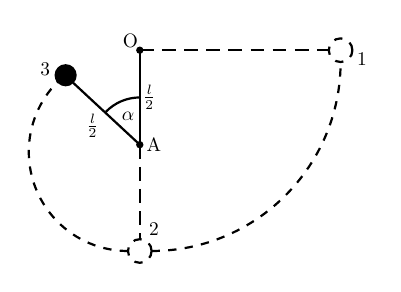
\begin{tikzpicture}[thick,scale=0.6, every node/.style={scale=0.7}]

    % Def. koordinaadid
    \coordinate (O) at (0,0) ;
    \coordinate (1) at (4,0) ;
    \coordinate (A) at (0,-2) ;
    \coordinate (2) at (0,-4);
    \coordinate (3) at (-1.41,-0.69);

    % Jooned, t2pid
    \draw[dash pattern=on5pt off3pt] (O) -- (1);
    \draw[dash pattern=on5pt off3pt] (A) -- (2);
    \draw[thick,dashed] (4.25,0) circle (0.25cm);
    \draw[thick,dashed] (0,-4.25) circle (0.25cm);
    \draw[thick] (O) -- (A);
    \draw[thick] (A) -- (3);
    \filldraw [black] (A) circle (1.5pt);
    \filldraw [black] (O) circle (1.5pt);
    \filldraw [black] (-1.57,-0.53) circle (6pt);
    
    

    % Nurgad ja punktid
    \draw (0,-1) arc (90:136:1);
    \draw[thick, dashed] (0.25,-4.25) arc (270:360:4);
    \draw[thick, dashed] (-0.25,-4.25) arc (270:135:2.1);
    \node[] at (-0.25,-1.4)  {$\alpha$};
    \node[] at (4.7,-0.2)  {$1$};
    \node[] at (0.3,-3.8)  {$2$};
    \node[] at (-2.0,-0.4)  {$3$};
    \node[] at (-0.2,0.2)  {O};
    \node[] at (0.3,-2)  {A};
    \node[] at (0.2,-1)  {$\frac{l}{2}$};
    \node[] at (-1,-1.6)  {$\frac{l}{2}$};
\end{tikzpicture}
\end{wrapfigure}

Punktis O kinnitatud niidi pikkusega $l$ otsas ripub väike kuulike. Kuulike viiakse kõrvale ja vabastatakse tõuketa asendist 1. Kuuli jõudes asendisse 2, kohtab niit joonise tasandiga risti olevat varrast punktis A, mis asub punktist O kaugusel $l/2$ sellega samal vertikaalil. Leida, millise nurga $\alpha$ väärtuse korral niidi pinge $T=0$ (asend 3). Õhutakistust ja hõõrdumist vardal arvestama ei pea.
\fi


\ifHint
Niidis kaob tõmbejõud, kui raskusjõu niidisuunaline komponent saab võrdseks tsentrifugaaljõuga. Kuuli kiirus asendis 3 on leitav energia jäävuse seadusest.
\fi


\ifSolution
Niidis kaob tõmbejõud, kui raskusjõu niidisuunaline komponent saab võrdseks tsentrifugaaljõuga. Märgistame nurga niidi ning horisontaaljoone vahel $\theta$-ga. Tsentrifugaaljõud avaldub kui $F_t=mv^2/r=2mv^2/l$ ning raskusjõu niidisuunaline komponent $F_rn=mg\sin\theta$. Need peavad võrduma, seega:
$$\frac{2mv^2}{l}=mg\sin\theta \Rightarrow v^2=\frac{gl\sin\theta}{2}.$$
Võttes potentsiaalse energia nivoo nullpunktiks asendi 2, saame et kuuli energia asendis 1 on $E_1=mgl$. Asendis 3 on aga kuulikese energia $E_3=mv^2/2+mg(1+\sin\theta)l/2$. Kuna kehtib energia jäävuse seadus, peab kehtima $E_1=E_3$:
$$mgl=\frac{mv^2}{2}+mg(1+\sin\theta)\frac{l}{2} \Rightarrow v^2=gl(1-\sin\theta).$$
Pannes kaks avaldist $v^2$ jaoks omavahel võrduma, saame:
$$\frac{gl\sin\theta}{2}=gl(1-\sin\theta)\Rightarrow \frac{3}{2}\sin\theta=\frac{3}{2}\cos\alpha=1 \Rightarrow \alpha=\arccos\frac{2}{3}.$$
\fi


\ifEngStatement
% Problem name: Pendulum with two parts
\begin{wrapfigure}[10]{r}{0.4\textwidth}
\vspace{-5pt}
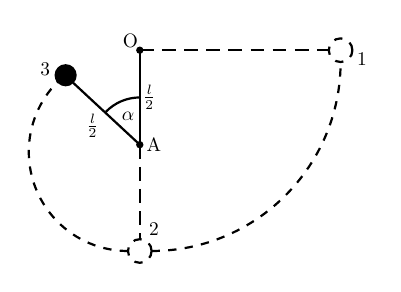
\begin{tikzpicture}[thick,scale=0.6, every node/.style={scale=0.7}]

    % Def. koordinaadid
    \coordinate (O) at (0,0) ;
    \coordinate (1) at (4,0) ;
    \coordinate (A) at (0,-2) ;
    \coordinate (2) at (0,-4);
    \coordinate (3) at (-1.41,-0.69);

    % Jooned, t2pid
    \draw[dash pattern=on5pt off3pt] (O) -- (1);
    \draw[dash pattern=on5pt off3pt] (A) -- (2);
    \draw[thick,dashed] (4.25,0) circle (0.25cm);
    \draw[thick,dashed] (0,-4.25) circle (0.25cm);
    \draw[thick] (O) -- (A);
    \draw[thick] (A) -- (3);
    \filldraw [black] (A) circle (1.5pt);
    \filldraw [black] (O) circle (1.5pt);
    \filldraw [black] (-1.57,-0.53) circle (6pt);
    
    

    % Nurgad ja punktid
    \draw (0,-1) arc (90:136:1);
    \draw[thick, dashed] (0.25,-4.25) arc (270:360:4);
    \draw[thick, dashed] (-0.25,-4.25) arc (270:135:2.1);
    \node[] at (-0.25,-1.4)  {$\alpha$};
    \node[] at (4.7,-0.2)  {$1$};
    \node[] at (0.3,-3.8)  {$2$};
    \node[] at (-2.0,-0.4)  {$3$};
    \node[] at (-0.2,0.2)  {O};
    \node[] at (0.3,-2)  {A};
    \node[] at (0.2,-1)  {$\frac{l}{2}$};
    \node[] at (-1,-1.6)  {$\frac{l}{2}$};
\end{tikzpicture}
\end{wrapfigure}
A thread of length $l$ is fixed to a point O and a small ball is hanging at the end of the thread. The ball is brought to the side and is released at the position 1 without additional force. When the ball reaches the position 2 the thread meets a rod at the point A, the rod is perpendicular to the drawing’s plane. In the same vertical the point A is at a length $l/2$ from the point O. Find for what value of $\alpha$ is the thread’s tension $T=0$ (position 3). Do not account for air resistance or friction.
\fi


\ifEngHint
The pulling force in the thread disappears if the gravity force’s component with the same direction as the thread will be equal to the centrifugal force. The ball’s speed in the position 3 can be found from the conservation of energy.
\fi


\ifEngSolution
The pulling force disappears in the thread if gravity force’s component with the same direction as the thread gets equal to centrifugal force. Let us mark the angle between the thread and the horizontal line as $\theta$. The centrifugal force is expressed as $F_t=mv^2/r=2mv^2/l$ and the gravity force’s component with the thread’s direction as $F_rn=mg\sin\theta$. These have to be equal, thus:
$$\frac{2mv^2}{l}=mg\sin\theta \Rightarrow v^2=\frac{gl\sin\theta}{2}.$$ 
Taking the position 2 as the zero point of potential energy we get that the energy of the ball in the position 1 is $E_1=mgl$. In the position 3, however, the energy of the ball is $E_3=mv^2/2+mg(1+\sin\theta)l/2$. Because the conservation of energy applies, $E_1=E_3$ must apply:
$$mgl=\frac{mv^2}{2}+mg(1+\sin\theta)\frac{l}{2} \Rightarrow v^2=gl(1-\sin\theta).$$ 
If we equalize the two equations for $v^2$ we get:
$$\frac{gl\sin\theta}{2}=gl(1-\sin\theta)\Rightarrow \frac{3}{2}\sin\theta=\frac{3}{2}\cos\alpha=1 \Rightarrow \alpha=\arccos\frac{2}{3}.$$
\fi
}